\documentclass[11pt, ngerman]{article}
\usepackage{tikz-network}
\usepackage[left=2.5cm, right = 2.5cm,top=2cm,bottom=2.5cm]{geometry}
\usepackage{babel}

\title{\Huge Aufgabe 3: Pancake Sort}
\author{\Large Finn Rudolph \\ \\ \Large Teilnahme-ID: 67571}
\date{\Large 23. Dezember 2022}

\begin{document}

\begin{titlepage}
    \maketitle
\end{titlepage}

\tableofcontents

\section{Lösungsidee}

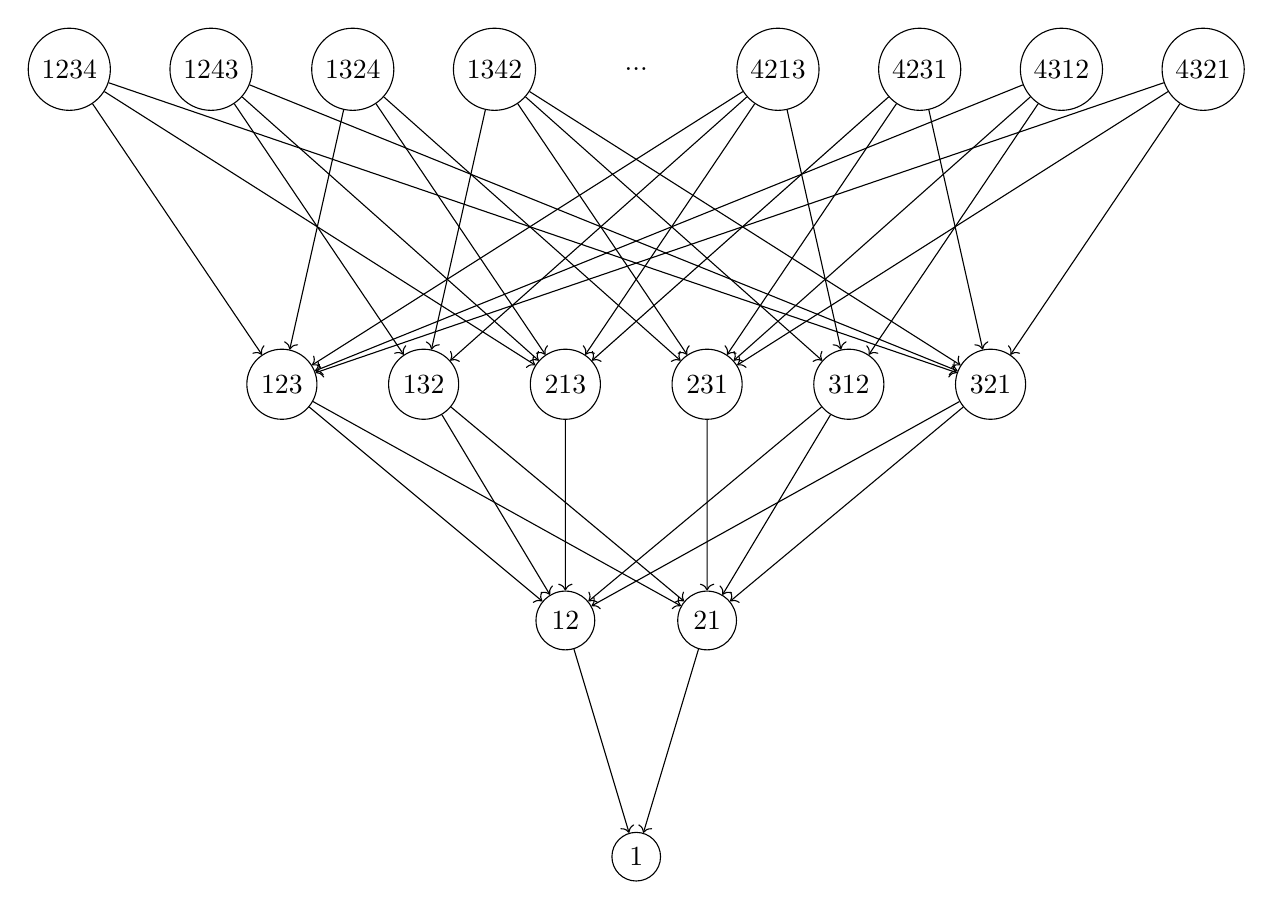
\begin{tikzpicture}[node distance = {18mm}, main/.style = {draw, circle}]
    \node[main](1234) at (0, 14) {1234};
    \node[main](1243) [right of = 1234] {1243};
    \node[main](1324) [right of = 1243] {1324};
    \node[main](1342) [right of = 1324] {1342};

    \node[](d) [right of = 1342] {...};
    \node[main](4213) [right of = d] {4213};
    \node[main](4231) [right of = 4213] {4231};
    \node[main](4312) [right of = 4231] {4312};
    \node[main](4321) [right of = 4312] {4321};

    \node[main](123) at (2.7, 10) {123};
    \node[main](132) [right of = 123] {132};
    \node[main](213) [right of = 132] {213};
    \node[main](231) [right of = 213] {231};
    \node[main](312) [right of = 231] {312};
    \node[main](321) [right of = 312] {321};

    \node[main](12) at (6.3, 7) {12};
    \node[main](21) [right of = 12] {21};

    \node[main](1) at (7.2, 4) {1};

    \draw[->](1234) -- (123);
    \draw[->](1234) -- (213);
    \draw[->](1234) -- (321);

    \draw[->](1243) -- (132);
    \draw[->](1243) -- (213);
    \draw[->](1243) -- (321);

    \draw[->](1324) -- (213);
    \draw[->](1324) -- (123);
    \draw[->](1324) -- (231);

    \draw[->](1342) -- (231);
    \draw[->](1342) -- (132);
    \draw[->](1342) -- (312);
    \draw[->](1342) -- (321);

    \draw[->](4213) -- (213);
    \draw[->](4213) -- (312);
    \draw[->](4213) -- (132);
    \draw[->](4213) -- (123);

    \draw[->](4231) -- (231);
    \draw[->](4231) -- (321);
    \draw[->](4231) -- (213);

    \draw[->](4312) -- (312);
    \draw[->](4312) -- (231);
    \draw[->](4312) -- (123);

    \draw[->](4321) -- (321);
    \draw[->](4321) -- (231);
    \draw[->](4321) -- (123);

    \draw[->](123) -- (12);
    \draw[->](123) -- (21);
    \draw[->](132) -- (21);
    \draw[->](132) -- (12);
    \draw[->](213) -- (12);
    \draw[->](231) -- (21);
    \draw[->](312) -- (12);
    \draw[->](312) -- (21);
    \draw[->](321) -- (12);
    \draw[->](321) -- (21);

    \draw[->](12) -- (1);
    \draw[->](21) -- (1);
\end{tikzpicture}

\end{document}